%!TeX program = xelatex
\documentclass[a4paper]{article}
\usepackage{graphicx}
\usepackage{amsmath, amsfonts, geometry, float, listings, enumerate, multicol}
\usepackage{multicol, float, color, colortbl}
\usepackage{tikz, titlesec, parskip, pgfplots, filecontents}
\usepackage{hyperref}
\usepackage{amsmath}
\usepackage{tikz, titlesec, parskip}
\usepackage{tikz,pgfplots}
\usepackage[americanvoltages,fulldiodes,siunitx]{circuitikz}
\usetikzlibrary{shapes,arrows}
\usetikzlibrary{angles,quotes}
\usepackage{enumitem}

\titlespacing{\section}{0pt}{10pt}{0pt}
\titlespacing{\subsection}{0pt}{10pt}{0pt}
\titlespacing{\subsubsection}{0pt}{10pt}{0pt}

\usetikzlibrary{calc,patterns,through}
\newcommand{\arcangle}{%
	\mathord{<\mspace{-9mu}\mathrel{)}\mspace{2mu}}%
}

\renewcommand{\baselinestretch}{1.4}
 \geometry{
 a4paper,
 total={170mm,257mm},
 left=20mm,
 top=20mm,
 }
\usepackage{fancyhdr}
\usepackage{indentfirst}
\pagestyle{fancy}
\fancyhf{}
\rhead{\textbf{آمار و احتمال مهندسی}}
\lhead{\textbf{تمرین عملی سری اول}}
\cfoot{(\space \space \space \space \textbf{\thepage}  \space \space \space)}
\renewcommand{\headrulewidth}{1pt}
\renewcommand{\footrulewidth}{1pt}

 
\usepackage{xepersian}
\setlatintextfont{Times New Roman}
\settextfont{XB Niloofar}
\DefaultMathsDigits

\makeatletter
\bidi@patchcmd{\@Abjad}{آ}{الف}
{\typeout{Succeeded in changing آ into الف}}
{\typeout{Failed in changing آ into الف}}
\makeatother
\PersianAlphs

\begin{document}
\begin{minipage}{0.6\textwidth}
\begin{bf}
\begin{center}
	به نام خدا\\
	\vspace{0.25cm}
	دانشگاه صنعتی شریف\\
	\vspace{0.25cm}
	دانشکده مهندسی برق\\
	\vspace{0.5cm}

\large
گروه دکتر کرباسی - آمار و احتمال مهندسی \\
نیم سال دوم
۱۴۰۱-۱۴۰۰\\
\Large
\vspace{0.4cm}
تمرین عملی سری اول \\
\end{center}
\end{bf}
\normalsize
\end{minipage} \hfill
\begin{minipage}{0.35\textwidth}
\begin{flushleft}

\includegraphics[width=0.6\textwidth]{Shariflogo.png}\\ \large
\end{flushleft}

 \end{minipage}
\\

\rule[0.1\baselineskip]{\textwidth}{1.5pt}

\large

\section*{
لطفاً به نکات زیر توجه بفرمایید: (رعایت نکردن این موارد باعث کاهش نمره می‌شود.)
}
\begin{enumerate}
	\item 
نتایج و پاسخ های خود را در یک فایل با فرمت zip به نام
\LR{HW$1$\_StudentID\_Name}
 در سایت  
\href{https://quera.org/overview/add_to_course/course/10631}{\lr{Quera}} 
 قرار دهید. همچنین فایل پایتون خود را به همان نام در قسمت مخصوص به خود آپلود کنید.
	\item 
کسب نمره کامل در هر سؤال مستلزم تحویل  \textbf{کدها} و \textbf{توضیحات} می‌باشد. 
\item 
برای سؤالات، باید روشی که استفاده کرده‌اید را توضیح  و نتایجی که گرفته‌اید را ارائه دهید. این توضیحات می‌تواند در یک فایل  .pdf  و یا در یک فایل  .ipynb باشد. 
\item 
کدهای خود را خوانا بنویسید و کامنت‌‌گذاری کنید. در plot های خود عنوان، label و خط‌کشی‌های مناسب را اضافه کنید.
\item
در طول ترم امکان ارسال با تاخیر پاسخ  همه‌ی تمارین تا سقف پنج روز و در مجموع دوازده روز وجود دارد. پس از گذشت این مدت، پاسخ‌های ارسال‌شده پذیرفته نخواهند بود. همچنین، به ازای هر روز تأخیر غیر مجاز  بیست درصد از نمره تمرین به صورت ساعتی کسر خواهد شد.
\item 
کدهای شما تماماً باید توسط خودتان نوشته شده باشند. هرگونه استفاده از کد دیگران به هر شکل ممکن، تقلب محسوب می‌شود و نمره تمرین کامپیوتری جاری صفر خواهد شد. پس در هیچ صورت کدهای خود را برای دیگران ارسال نکنید.
\item 
ابهام يا اشكالات خود را مي توانيد  از طریق
\href{mailto:smmzdr@gmail.com}{\LR{Smmzdr@gmail.com}}
یا 
\href{mailto:javadiamirhosein.2000@gmail.com}{\LR{Javadiamirhosein.$2000$@gmail.com}}
مطرح نماييد.
\item 
مهلت تحویل:  
\end{enumerate}
\rule[0.1\baselineskip]{\textwidth}{1.5pt}

\clearpage
\section{مسئله سوزن بوفون}
فرض کنید یک سطح داریم که روی آن خطوط موازی به فواصل $ 5 $ سانتی‌متری کشیده‌ایم. سوزنی به طول $ 1 $ سانتی‌متر را $ 100000 $ بار به‌طور تصادفی روی این سطح می‌اندازیم و 
نسبت تعداد دفعاتی که سوزن یکی از آن خطوط را قطع می‌کند به کل دفعات را به دست می‌آوریم. با توجه به این نسبت، تخمین خود از عدد 
$ \pi $
را اعلام کنید. 
\\
برای شبیه‌سازی این مسئله به دو پارامتر $ x $ و $ \theta $ نیاز دارید که به ترتیب $ x $ از مختصات مرکز سوزن و $ \theta $ از زاویه‌ی سوزن با خطوط به دست می‌آید. $ x $ را به صورت یونیفرم از بازه‌ی
 $ (0,5) $
 و $ \theta $ را به صورت یونیفرم از بازه‌ی 
 $ (0,\pi) $
 انتخاب ‌کنید.
\\
توابع پیشنهادی:
\lr{np.random.uniform}
از کتاب‌خانه‌ی 
\lr{numpy}

\vspace{0.5cm}
\section{متغیرهای تصادفی و تحقق‌هایش}
‌شبیه‌سازی مونت کارلو مدل احتمالاتی برای پیش‌بینی احتمال نتایج مختلف در یک فرآیند تصادفی است. در این مدل، احتمال با تعریف فرکانسی به صورت زیر تقریب زده ‌می‌شود. 
\begin{equation}
	\mathbb{P}(A) = \frac{\text{\lr{Number of times A happens}}}{\text{\lr{Total number of trials}}}
\end{equation}
با زیاد شدن تعداد دفعات تکرار آزمایش، خطای تقریب بالا را با احتمال خوبی از هر مقداري کمتر می‌شود. در این سوال قصد داریم با نمونه برداری از متغیر تصادفی، احتمالات دلخواهمان را به دست بیاوریم. 

یک خانه برای جلوگیری از دزدی، یک زنگ خطر نصب کرده‌است. احتمال رخ دادن دزدی و روشن شدن این زنگ بر حسب وجود دزد به ترتیب به شکل جدول
\ref{Pb}
و
\ref{Pab}
است. هر آزمایش تصادفی، یک زوج مرتب به شکل 
$ (x,y) $
است که $ x $ وقوع دزدی را مدل می‌کند و $ y $ روشن شدن یا نشدن زنگ‌ خطر را مشخص می‌کند. در هر آزمایش اول $ x $ را تعیین کنید و بر حسب $ x $ میتوانید برای $ y $ نمونه‌برداری کنید. با انجام حداقل $ 100000 $ آزمایش احتمالات زیر را به دست بیاورید و با مقدار واقعی‌شان مقایسه کنید.
\begin{itemize}
	\item $ \mathbb{P}(A = +a | B = +b) $
	\item $ \mathbb{P}(A = +a | B = -b) $ 
	\item $ \mathbb{P}(A = -a) $
\end{itemize}
توابع پیشنهادی:
\lr{np.random.randint}
از کتاب‌خانه‌ی 
\lr{numpy}
\\
\begin{minipage}{0.50 \linewidth}
	\centering
	\begin{figure}[H]
		\centering
		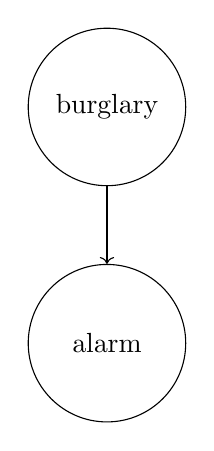
\begin{tikzpicture}[main/.style = {draw, circle, minimum width=20mm, minimum height=20mm}] 
			\node (1) [main]  at (3,6) {alarm};
			\node (2) [main]  at (3,9) {burglary};
			\draw[->]  (2) -- (1) node[midway,above] {};
		\end{tikzpicture} 
	\caption{Model}
	\end{figure}
\end{minipage}
\begin{minipage}{0.50 \linewidth}
\begin{figure}[H]
	\centering
		\begin{tabular}{| c | c |}
		\hline	
		$ \mathbb{P}(B) $ & $ B $  \\
		\hline	
		$ 0.01 $ & $ +b $\\
		\hline	
		$ 0.99 $ & $ -b $ \\
		\hline  
	\end{tabular}
	\caption{\lr{Probability of burglary}}
	\label{Pb}
	\vspace{0.4cm}
	\begin{tabular}{| c | c | c |}
		\hline	
		$ \mathbb{P}(A|B) $ & $ A $ & $ B $  \\
		\hline	
		$ 0.94 $ & $ +a $ & $ +b $  \\
		\hline	
		$ 0.06 $ & $ -a $ & $ +b $  \\
		\hline
		$ 0.01 $ & $ +a $ & $ -b $  \\
		\hline
		$ 0.99 $ & $ -a $ & $ -b $  \\
		\hline  
	\end{tabular}
	\caption{\lr{Probability of alarm given burglary}}
	\label{Pab}
\end{figure}
\end{minipage}
\newpage
\section{مثلث های مرکزدوست!}
در این سوال نیز قصد داریم با استفاده از شبیه سازی مونت کارلو یک مساله جالب را حل کنیم. دایره ای را در نظر بگیرید که روی محیط آن
$n \geq 3$
نقطه که رئوس یک $n$ ضلعی منتظم هستند قرار دارند. مثلث هایی که با این نقاط میتوان ساخت را در نظر بگیرید، آن دسته از مثلث هایی که مرکز دایره درونشان قرار دارد را مثلث های مرکزدوست می نامیم. قصد داریم بدانیم که با بزرگتر شدن
$n$
احتمال اینکه با انتخاب سه نقطه دلخواه از این 
$n$
نقطه یک مثلث مرکزدوست ایجاد شود به چه مقداری میل میکند. 
\\
\begin{figure}[H]
\centering
	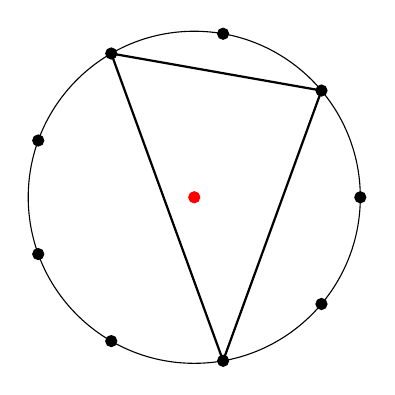
\begin{tikzpicture}[x = 1pt, y = 1pt]
		\draw (0,0) circle (60);
		\filldraw[red] (0,0) circle (2);
		\filldraw[black] ({60*cos(40)},{60*sin(40)}) circle (2);
		\filldraw[black] ({60*cos(80)},{60*sin(80)}) circle (2);
		\filldraw[black] ({60*cos(120)},{60*sin(120)}) circle (2);
		\filldraw[black] ({60*cos(160)},{60*sin(160)}) circle (2);
		\filldraw[black] ({60*cos(200)},{60*sin(200)}) circle (2);
		\filldraw[black] ({60*cos(240)},{60*sin(240)}) circle (2);
		\filldraw[black] ({60*cos(280)},{60*sin(280)}) circle (2);
		\filldraw[black] ({60*cos(320)},{60*sin(320)}) circle (2);
		\filldraw[black] ({60*cos(360)},{60*sin(360)}) circle (2);
		\draw[black, thick] ({60*cos(40)},{60*sin(40)}) -- ({60*cos(120)},{60*sin(120)});
		\draw[black, thick] ({60*cos(280)},{60*sin(280)}) -- ({60*cos(120)},{60*sin(120)});
		\draw[black, thick] ({60*cos(40)},{60*sin(40)}) -- ({60*cos(280)},{60*sin(280)});
	\end{tikzpicture}
	\caption{یک مثلث مرکزدوست در حالتی که $n = 9$ است}
\end{figure}

\begin{enumerate}
	\item
ابتدا تابعی بنویسید که با ورودی گرفتن
$n$
سه نقطه تصادفی از نقاط روی دایره را در نظر بگیرد و چک کند که مثلث ساخته شده با این سه  نقطه مرکزدوست میباشد یا خیر و این آزمایش را $10000$ بار تکرار کند، سپس با استفاده از روش مونت کارلو احتمال مرکزدوست بودن مثلث برای $n$ مورد نظر را در خروجی برگرداند.
	\item
تابع دیگری بنویسید که تابع قسمت قبل را برای
$3 \leq n \leq 1500$
اجرا کند و حاصل را در آرایه ای به نام 
\lr{MC\_Result}
ذخیره کند. سپس آرایه ای به نام
\lr{MC\_Avg}
تعریف کنید که عضو $i$ ام آن برابر میانگین $i$ عضو اول آرایه
\lr{MC\_Result}
باشد و این آرایه را به عنوان خروجی تابع برگردانید.(در حقیقت اگر قرار باشد با بزرگتر شدن $n$ احتمال مرکزدوست بودن مثلث ساخته شده به عددی خاص میل کند باید میانگین این احتمال ها نیز به آن عدد میل کند، این کار را جهت کم کردن نوسانات نموداری که قرار است در ادامه چاپ کنیم انجام میدهیم)
	\item
خروجی تابع فوق را در یک نمودار رسم کنید. با بزرگتر شدن $n$، احتمال اینکه با انتخاب سه نقطه تصادفی یک مثلث مرکزدوست داشته باشیم به چه مقداری میل میکند؟(برای این قسمت میتوانید آخرین عضو خروجی قسمت قبل را چاپ کنید) از این موضوع چه نتیجه ای می توان گرفت؟
	\item
(
\textcolor{red}{\textbf{امتیازی}}
)
از روش تئوری ثابت کنید اگر دایره دلخواهی داشته باشیم و سه نقطه تصادفی روی محیط آن انتخاب کنیم، احتمال اینکه مثلثی که این سه نقطه رئوس آن هستند مرکز دایره را شامل بشود
$\frac{1}{4}$
است. (راهنمایی: مسئله را به صورت انتخاب یک نقطه تصادفی و دو قطر تصادفی از دایره مدلسازی کنید)
\\
\end{enumerate}
توابع پیشنهادی:
\lr{random.sample}
از کتاب‌خانه‌ی 
\lr{random}
و 
\lr{matplotlib.pyplot.plot}
از کتاب‌خانه‌ی
\lr{matplotlib}
\end{document}
